\documentclass{article}
\usepackage[utf8]{inputenc}

\title{MATH3160 — Portfolio 6.3}
\author{Mike Medved}
\date{November 29th, 2022}

\usepackage{color}
\usepackage{amsthm}
\usepackage{amssymb} 
\usepackage{amsmath}
\usepackage{listings}
\usepackage[margin=1in]{geometry} 
\usepackage[dvipsnames]{xcolor}
\usepackage{tikz}

\newtheorem*{thm}{Theorem}

\begin{document}

\maketitle

\section{Deliverables}

\subsection{Standard Normal Random Variable}

\begin{figure}[!htb]
    \begin{minipage}[b]{0.5\textwidth}
        \centering
        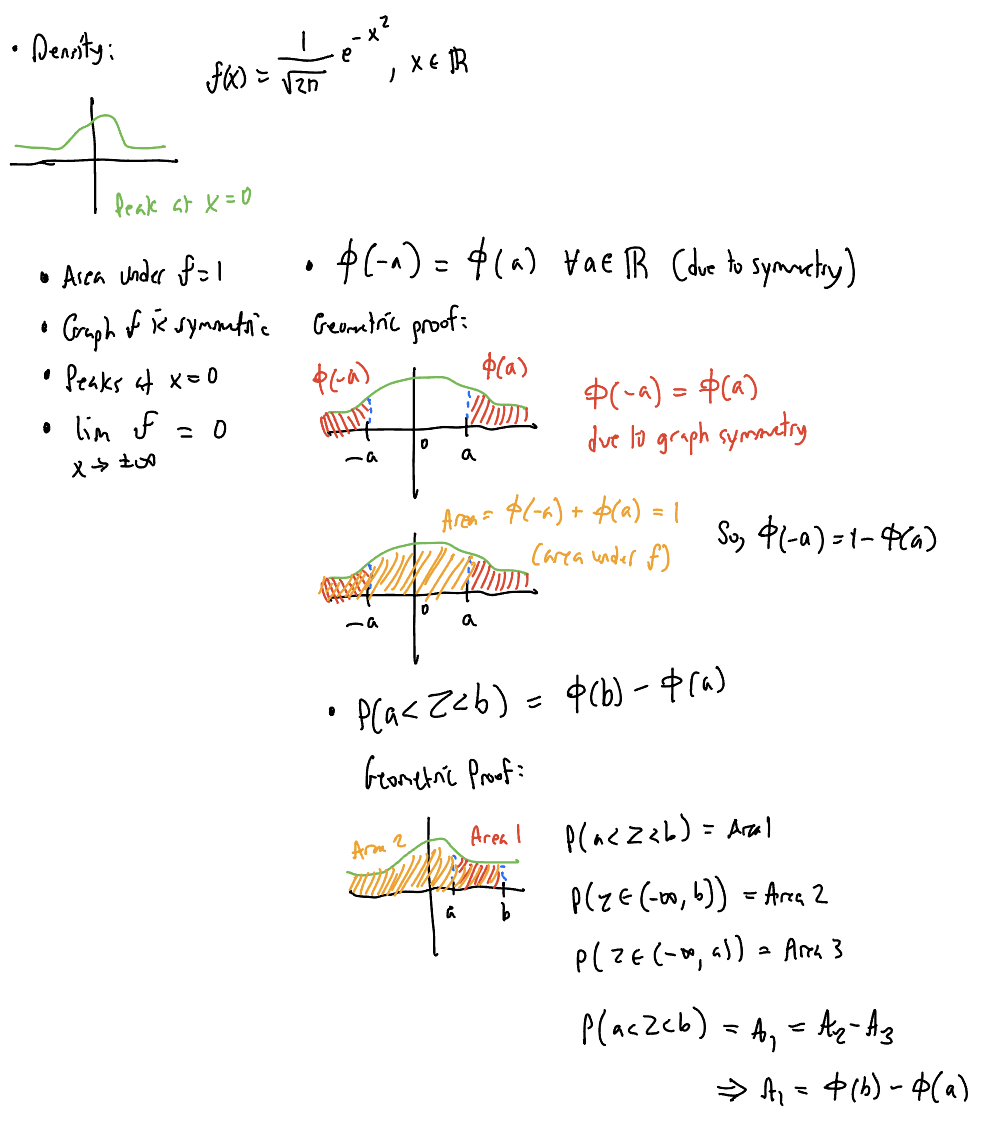
\includegraphics[scale=0.25]{q1.jpeg}
    \end{minipage}
    \begin{minipage}[b]{0.5\textwidth}
        \centering
        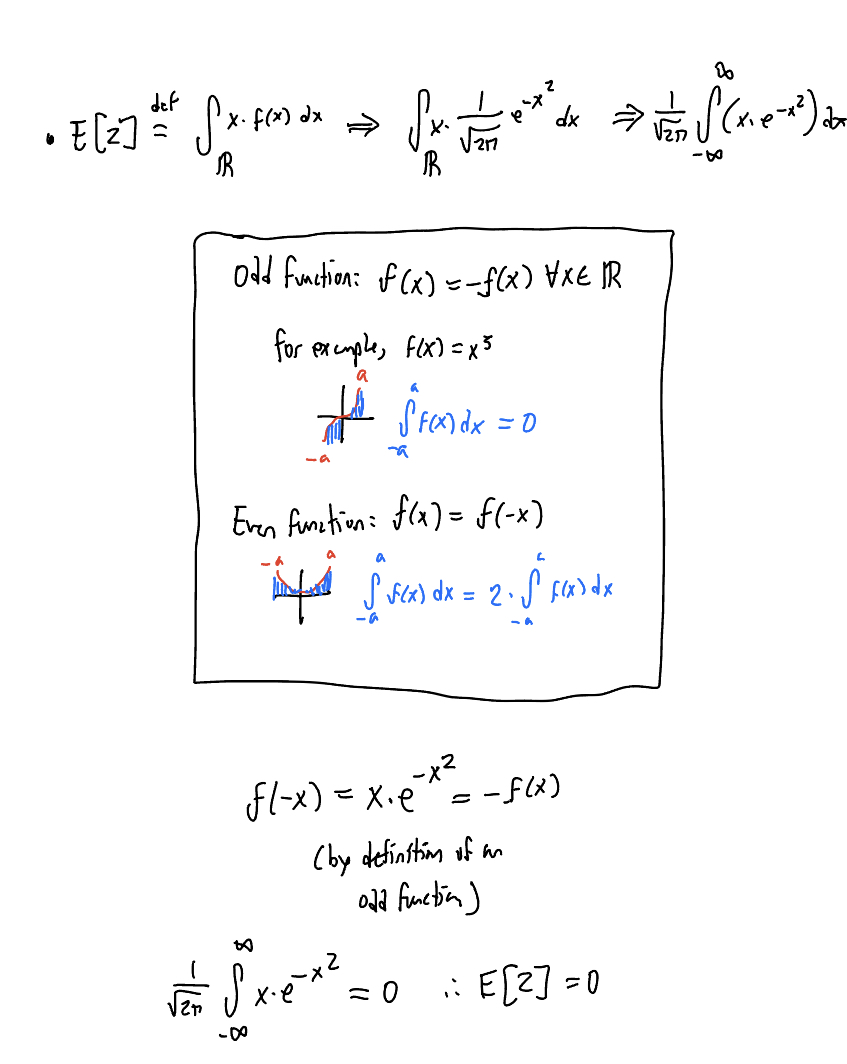
\includegraphics[scale=0.25]{q1-2.jpeg}
    \end{minipage}
\end{figure}

\begin{center}
    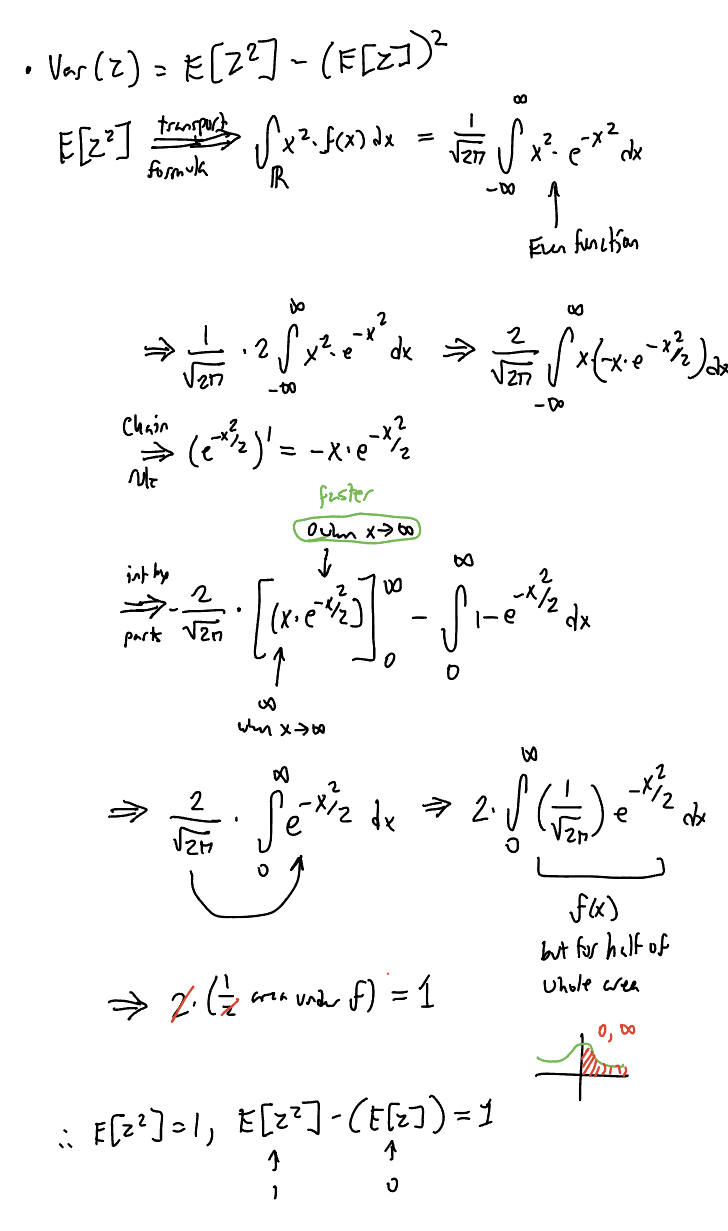
\includegraphics[scale=0.25]{q1-3.jpeg}
\end{center}

\subsection{General Normal $\rightarrow$ Standard Normal}

Let $X \sim \mathcal{W}(\mu, \sigma^2)$, then $\frac{x-\mu}{\sigma} \sim \mathcal{N}(0,1)$. This is called the reduction to a standard normal random variable, and can be accomplished by transforming the random variable $X$ into a standard normal random variable $Z$ by the above reduction.

$\hfill \break$
The opposite holds, given $Z \sim \mathcal{N}(0,1)$, we can transform $Z$ into a random variable $X$ with a general normal distribution by the following transformation to revert back to a general normal random variable:

\begin{equation*}
    X = \mu + \sigma Z
\end{equation*}

\newpage
\subsection{General Normal Random Variable}

\begin{center}
    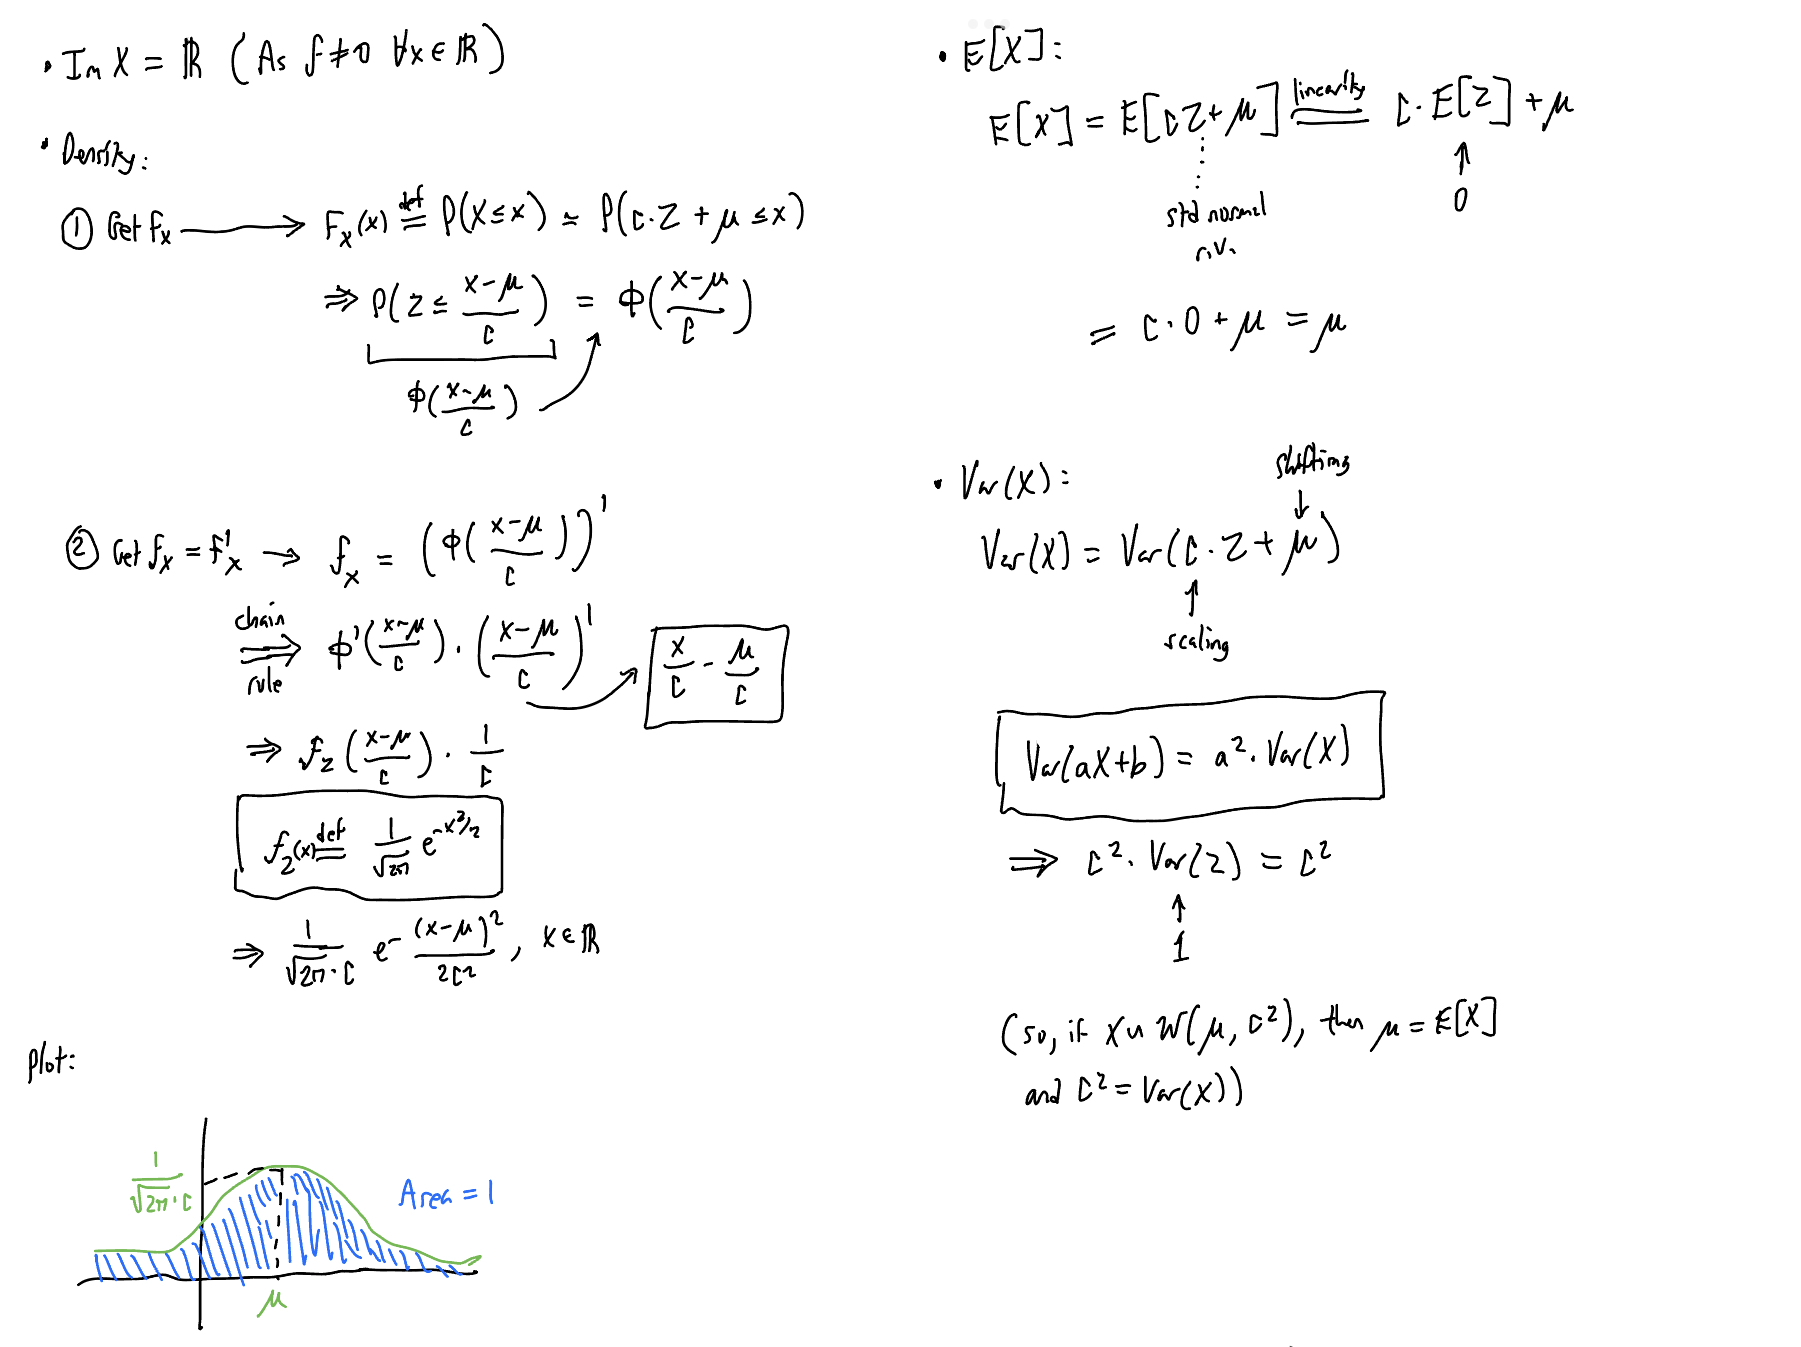
\includegraphics[scale=0.25]{q3.jpeg}
\end{center}

\end{document}